\documentclass{beamer}
\usepackage[utf8]{inputenc}
\usepackage[brazil]{babel}
\usepackage{xcolor}
\usepackage{tikz}
\usetikzlibrary{positioning,calc}
\usepackage{graphicx}
\usepackage{cite}
\usepackage{hyperref}
\usepackage{array}
\usepackage{amsmath}
\usepackage{amssymb}
\usepackage{amsthm}
\usepackage{listings}
\usepackage{fontawesome}
\usepackage{caption}
\usepackage{subcaption}
\usepackage{wrapfig}
\usetheme{mtmufsc} %%%%%%%%Use this template
\renewcommand{\qedsymbol}{$\blacksquare$}
\usepackage[alf]{abntex2cite}

\newtheorem{teo}{Teorema}[section]
\newtheorem{prop}{Proposição}[section]
\theoremstyle{definition}
\newtheorem{exem}{Exemplo}[section]
\newtheorem{defin}{Definição}[section]
\newtheorem{obs}{Observação}[section]


% This is a beamer template inspired by unofficial Oxford University Beamer Template, made by Clara Eleonore Pavillet.
\title{O poder da Aprendizagem Profunda Parte 2: \\
Os polinômios atacam novamente}
\author{Felipe Kaminsky Riffel}
\date{\today}
\institute{Universidade Federal de Santa Catarina}

\begin{document}

{\setbeamertemplate{footline}{} 
\frame{\titlepage}}
% \frame{}

\begin{frame}{Sumário}
    \tableofcontents
\end{frame}
  
% %Sempre que iniciar uma nova sessão, você pode fazer um slide de transição com o índice.
% \begin{frame}
% \tableofcontents[currentsection]
% \end{frame}

\section{Artigo: Power of Deep Learning on Expressing Natural Functions}    
\begin{frame}
\tableofcontents[currentsection]
\end{frame}

\begin{frame}{Why does deep and cheap learning work so well?}

    Artigo: \\
    
    TEGMARK, Max; ROLNICK, David. The Power of Deeper Networks for Expressing Natural Functions. arXiv. 2018. \cite{rolnick2018}

    \vspace{1em}
    Artigo submetido para apresentação na modalidade pôster para o International Conference on Learning Representations (ICLR) 2018.

\end{frame}

\section{Introdução}

\section{O poder da Aproximação}
\begin{frame}
    \tableofcontents[currentsection]
\end{frame}

\begin{frame}{Definições}
    \small

    \begin{defin}
        Consideramos o modelo de redes neurais feedforward ou multilayer perceptron:
        \begin{equation}
            N(x) = A_k \circ \sigma \circ A_{k-1} \circ \cdots \sigma A_1 \sigma A_0 x
        \end{equation}
        onde:
        \begin{itemize}
            \item $A_i:\mathbb R^{n_i} \to \mathbb R^{n_{i+1}}$ são matrizes/operadores afins;
            \item $\sigma:\mathbb R^{n_i} \to \mathbb R^{n_i}$ são funções não lineares aplicados ponto a ponto;
        \end{itemize}
        \pause
        Denominamos:
        \begin{itemize}
            \item $k$ a profundidade da rede; \pause
            \item camadas escondidas cada vetor $\sigma A_i \sigma A_{i-1} \cdots A_0 x$; \pause
            \item neurônio as entradas de cada $\sigma A_i \sigma A_{i-1} \cdots A_0x$.
        \end{itemize}
    \end{defin}
\end{frame}

\begin{frame}{Definições}
    \small

    \begin{defin}
    Dado $\varepsilon>0$ e um compacto $K$, dizemos que uma rede $N(\mathbf x)$ $\varepsilon-$\textit{aproxima} uma função $f:\mathbb R^n \to \mathbb R^m$ se 
    \begin{equation*}
        \sup_{x \in K} |N(\mathbf x) - f(\mathbf x)|< \varepsilon
    \end{equation*}
    \end{defin}

    \pause 

    \begin{defin}
        Dizemos que uma rede $N(x)$ \textit{Taylor-aproxima} um polinômio $p(x)$, com $p:\mathbb R^n \to \mathbb R$ de grau $d$, se $p(x)$ é o polinômio de Taylor de grau $d$ de $N(x)$ em torno da origem. \pause I.e.,

        \begin{align*}
            N(x) &= \sum_{|\alpha| \leq d} \frac{D^{\alpha}N(0)x^\alpha}{\alpha!} + \mathcal O(x^d) \\
            &= p(x) + \mathcal O(x^d)
        \end{align*}
    \end{defin}

\end{frame}


\begin{frame}{Proposição 3.3}
    \begin{prop}
    Seja $p:\mathbb R^n \to \mathbb R$ polinômio homogêneo e suponha que a rede $N$ Taylor-aproxima $p$ em um compacto $K$. Então, para cada $\varepsilon>0$, existe uma rede $N_{\varepsilon}$ que $\varepsilon-$aproxima $p$, tais que $N$ e $N_\varepsilon$ tem o mesmo número de neurônios em cada camada.
    \end{prop}
\end{frame}

\begin{frame}{Prop 3.3 - Demonstração}
    \small

    Seja $p(x)$ polinômio de grau $d$.\pause Como $N$ Taylor-aproxima $p$, se $\sigma$ for inf. diferenciável:
    \begin{equation}
        N(x) = p(x) + E(x)
    \end{equation}
    com $\sum_{i=d+1}^\infty E_i(x)$ e cada $E_i$ homogêneo de grau $i$. \pause Assim,
    
    \begin{equation*}
        E_i(\delta x) = \delta^i E_i(x), \forall i \in \mathbb N.
    \end{equation*}

    \pause 

    Como $\sum_{i=d+1}^\infty E_i(x)<\infty, \forall x \in \mathbb R^n$, em particular, para $\delta<1$
    \begin{equation*}
        \sum_{i=d+1}^\infty E_i(\delta x) = \sum_{i=d+1}^\infty \delta^i E_i(x) <\infty
    \end{equation*}
    \pause de modo que
    \begin{equation*}
        \frac{1}{\delta^d} E(\delta x) = \sum_{i=d+1}^\infty \delta^{i-d} E_i(x) <\infty
    \end{equation*}
\end{frame}

\begin{frame}{Prop 3.3 - Demonstração}
    Como $i>d$, para $\delta$ suficientemente pequeno, cada $\delta^{i-d}$ se torna tão pequeno quanto queira, assim como $\frac{1}{\delta^d}E_i(\delta x) = \delta^{i-d} E_i(\delta x)$. Logo, $\frac{E(\delta x)}{\delta^d}$é arbitrariamente pequeno.

    \pause

    Seja $\varepsilon>0$ e tome $\delta$ t.q.
    \begin{equation}
        |\frac{E(\delta x)}{\delta^d} |<\varepsilon
    \end{equation}
    Defina $A_0' = \delta A_0$, $A_k' = \frac{1}{\delta^d} A_k \cdots A_0 (\delta x)$, \pause 
    \begin{align}
        N_\varepsilon(x) &= A_k' \sigma A_{k-1} \sigma \cdots \sigma A_1 \sigma A_0' x \\
        & = \frac{1}{\delta^d} A_k \sigma A_{k-1} \sigma \cdots \sigma A_1 \sigma (\delta A_0) x \\
        & = \frac{N(\delta x)}{\delta^d}
    \end{align}
\end{frame}


\begin{frame}{Prop 3.3 - Demonstração}

    Assim,

    \begin{align*}
        | N_\varepsilon(x) - p(x) | &= |\frac{1}{\delta^d} N(\delta x) - p(x)| \\
        &= |\frac{1}{\delta^d}(p(\delta x) + E(\delta x))-p(x)| \\
        &=|\frac{1}{\delta^d}p(\delta x) -p(x) + \frac{1}{\delta^d}E(\delta x) |
    \end{align*} \pause
    \begin{align*}
        &= |\frac{1}{\delta^d}E(\delta x)| < \varepsilon.
    \end{align*}
    Ou seja, $N_\varepsilon$ é $\varepsilon-$aproximação de $p$, como queríamos. $\square$
\end{frame}

\begin{frame}{Teorema 3.4}
    \begin{teo}
        Suponha que $p(x)$ é um polinômio de grau $d$ multivariado e que $\sigma_i := \sigma^{(i)}(0) \neq 0$, para cada $i\leq d$. Seja $m_k^\varepsilon(p)$ o número mínimo de neurônios em uma rede de profundidade $k$ que $\varepsilon-$aproxima $p$ em um compacto $K$. \pause 
        \vspace{1em}
        Então, o limite $\lim_{\varepsilon>0}m_k^\varepsilon(p)$ existe e é finito. 
    \end{teo}
\end{frame}

\begin{frame}{Teo. 3.4 - Demonstração}    
    Mostremos que $\lim_{\varepsilon \to 0} m_1^\varepsilon$ existe e é finito. \pause \vspace{1em}

    Sejam $p_1, \dots, p_s$ monômios t.q $p(x) = \sum_i^s p_i(x)$. Cada $p_i$ pode ser Taylor-aproximado por uma rede $N_i$ de 1 camada,conforme Teorema 2 de \citeonline{Lin2017}. 

    \pause
    \vspace{1em}

    Suponha que $N^i$ tem $m_i$ neurônios, tome $\varepsilon>0$ e seja $\delta = \frac{\varepsilon}{s}$. Pela Prop. 3.3, sendo $p_i$ homogêneo, existe uma rede $N^i_\delta$ que $\delta-$aproxima $N_i$.

    \pause
\end{frame}


\begin{frame}{Teo. 3.4 - Demonstração}
    Definimos:
    \begin{equation*}
        N_\varepsilon(x) = \sum_i N^i_\delta(x),
    \end{equation*}
    a qual tem $\sum_i m_i$ neurônios. \pause Então,

    \begin{align*}
        |N_\varepsilon(x) - p(x)| &= |\sum_i^s N^i_\delta(x)-\sum_i^s p_i(x)| \\
        &\leq \sum_i^s |N^i_\delta(x) - p_i(x)| \\
        &\leq \sum_i^s \frac{\varepsilon}{s} = \varepsilon.
    \end{align*}

    \pause

    Logo, $N_\varepsilon$ é uma $\varepsilon-$aproximação de $p$ com $\sum_m^i$ neurônios.
\end{frame}

\begin{frame}
    \frametitle{Teo. 3.4 - Demonstração}

    Na construção de $N_\delta^i$, o número de neurônios é o mesmo para cada $\delta$ escolhido. Isto é, $N_\delta$ tem sempre $\sum_i m_i$ neurônios, independente de $\delta$. \pause Portanto,

    \[
        m_1^\varepsilon(p) \leq \sum_i m_i, \forall \varepsilon>0.
    \]

    \pause
    Ou seja, $\lim_{\varepsilon\to 0} m_1^\varepsilon(p) \leq \infty$, como queríamos.

    \pause

    Podemos sempre construir uma rede $N_k$ de profundidade $k>1$ que aproxima uma rede $N_1(x)$ de uma camada:
    \begin{equation*}
        N_k(x) = A_k \sigma A_{k_1} \sigma \cdots A_2 \sigma N_1(x)
    \end{equation*}

    onde $A_i \sigma$ é uma camada de passagem, $\forall i>1$. \pause 
    
    Logo, $m_k(p)\lesssim m_1(p) < \infty$. $\blacksquare$. 
\end{frame}

\begin{frame}{Mínimos de Neurônios}
    \begin{defin}
        Seja $\sigma$ função não linear. Dado $p$ polinômio multivariado, seja $m_k^{uniform}(p)$ o número mínimo de neurônios em uma rede de profundidade $k$ que $\varepsilon-$aproxima $p$ para todo $\varepsilon>0$. \pause Denotamos:

        \begin{align*}
            m^{uniform}(p) = \min_{k \in \mathbb N} m_k^{uniform}(p)
        \end{align*}

        \pause

        I.e., é o mínimo de número de neurônios considerando todas as profundidades de redes.

        \pause

        \vspace{1em}

        Definimos $m_k^\text{Taylor}$ e $m^\text{Taylor}$ analogamente.
    \end{defin}
\end{frame}

\section{A ineficiência de redes mais rasas}
\begin{frame}
    \tableofcontents[currentsection]
\end{frame}

\begin{frame}{Teorema 4.1}
    
    \begin{teo}
        
        Seja $p(x)$ o monômio $p(x) = x_1^{r_1} x_2^{r_2} \cdots x_n^{r_n}$, com $d = \sum_{i=1}^{n} r_i$ e $\sigma$ função não linear qualquer. Suponha que $\sigma_i \neq 0$, para todo $i\leq 2d$. Então,
        \begin{itemize}
          \item[(i)] $m_1^{\text{uniform}}(p) = \prod_{i=1}^{n}(r_i + 1)$,
          \item[(ii)] $m^{\text{uniform}}(p) \leq \sum_{i=1}^{n} \left(7d\lceil \log_2(r_i) \rceil + 4\right)$,
        \end{itemize}
        onde $\lceil x \rceil$ denota o menor inteiro maior ou igual a $x$. 
    
    \end{teo}
\end{frame}

\begin{frame}{Teorema 4.2}
    
    \begin{teo}
        Seja $p(x)$ o monômio $p(x) = x_1^{r_1} x_2^{r_2} \cdots x_n^{r_n}$, com $d = \sum_{i=1}^{n} r_i$. e $\sigma$ função não linear qualquer. Suponha que $\sigma_i \neq 0$, para todo $i\leq d$. Então,
        \begin{itemize}
          \item[(i)] $m_1^{\text{Taylor}}(p) = \prod_{i=1}^{n}(r_i + 1)$,
          \item[(ii)] $m^{\text{Taylor}}(p) \leq \sum_{i=1}^{n} \left(7d\lceil \log_2(r_i) \rceil + 4\right)$.
        \end{itemize}
    
    \end{teo}
\end{frame}

\begin{frame}{Teorema 4.3}
    \begin{teo}
        Seja $p(x)$ um polinômio multivariado de grau $d$ e esparsidade $c$, com monômios $q_1(x), q_2(x), \dots, q_c(x)$. Seja $\sigma$ não linear e suponha que $\sigma_i \neq 0$, para todo $i\leq 2d$. Então, temos:
        \begin{itemize}
        \item[(i)] $m_1^{\text{uniform}}(p) \geq \frac{1}{c} \max_j m_1^{\text{uniform}}(q_j)$,
        \item[(ii)] $m^{\text{uniform}}(p) \leq \sum_j m^{\text{uniform}}(q_j)$.
        \end{itemize}

    \end{teo}
    
    \pause \textbf{Obs}: Dizemos que $p$ tem esparsidade $c$ se pode ser representado como a soma de $c$ monômios. 
    
    \pause \textbf{Obs2:} O resultado também é válido trocando $m^{uniform}$ para $m^{Taylor}$.
\end{frame}

\begin{frame}{Teorema 4.4}
    \begin{teo}
        Seja $p(x)$ o monômio $x_1^{r_1} x_2^{r_2} \cdots x_n^{r_n}$, com $d = \sum_{i=1}^{n} r_i$. Suponha que $\sigma_d \neq 0$ (os outros coeficientes de Taylor podem ser nulos). Então, $m_1^{\text{uniform}}(p)$ e $m_1^{\text{Taylor}}(p)$ são no mínimo $\frac{1}{d} \prod_{i=1}^{n}(r_i + 1)$. (Um limite inferior ainda melhor é o maior coeficiente no polinômio $\prod_i (1 + y + \cdots + y^{r_i})$.)
    \end{teo}
\end{frame}

\begin{frame}{Teorema 4.5}
    \begin{teo}
        Suponha que $\sigma_i \neq 0$ para cada $i \leq d$. Então, para cada polinômio $p(x)$ em uma variável de grau $d$,:
        \begin{equation*}
            m_1^{Taylor}(p) \leq d+1
        \end{equation*}
    \end{teo}
\end{frame}

\begin{frame}{Teo.4.5 - Demonstração}
    \small

    Sejam $a_0, a_1, \dots, a_n \in \mathbb R$ distintos. \pause Considere $A \in \mathbb R^{(d+1) \times (d+1)}$ dada por

    \begin{equation*}
        A_{ij} = a_i^j         
    \end{equation*}

    \pause \vspace{1em}

    Sabemos que $\det A \neq 0$ (matriz de Vandermond). Logo, $A$ é inversível. \pause Portanto, multiplicando as linhas de $A$ por um $b_i\neq 0$ produz outra inversível.

    \pause \vspace{1em}

    Sejam $A_i$ as colunas de $A$ e $\sigma(x) = \sum_j \sigma_j x_j$ expansão de Taylor de $\sigma$ em 0. Defina

    \begin{equation*}
        A' = \begin{bmatrix}
            |  & | & & | \\
            \sigma_0 A_0 & \sigma_1 A_1 & \cdots & \sigma_d A_d \\
            |  & | & & | 
        \end{bmatrix} = 
        \begin{bmatrix}
            1 & \sigma_1 a_1 & \cdots & \sigma_d a_1^n \\
            \vdots & \ddots & &  \vdots \\
            1 & \sigma_1 a_d & \cdots & \sigma_d a_d^n 
        \end{bmatrix}
    \end{equation*}
    
    \pause

    Por hipótese, $\sigma_i \neq 0$, portanto $A'$ é inversível.
\end{frame}

\begin{frame}{Teo 4.5 - Demonstração}
    \small
    \begin{equation}
        A' = \begin{bmatrix}
            |  & | & & | \\
            \sigma_0 A_0 & \sigma_1 A_1 & \cdots & \sigma_d A_d \\
            |  & | & & | 
        \end{bmatrix} = 
        \begin{bmatrix}
            1 & \sigma_1 a_1 & \cdots & \sigma_d a_1^n \\
            \vdots & \ddots & &  \vdots \\
            1 & \sigma_1 a_d & \cdots & \sigma_d a_d^n 
        \end{bmatrix}
    \end{equation}

    Note que cada linha $i$ de $A$ corresponde os coeficientes da expansão de Taylor de $\sigma(a_i x)$:
    \begin{equation*}
        \sigma(a_i x) = \sum_j^d \sigma_j (a_i x)^j = \sum_j^d \sigma_j a_i^j x^j.
    \end{equation*}

    \pause

    Sendo as linhas L.I., os polinômios:
    \begin{equation*}
        p_i(x) = \sum_j^d \sigma_i a_i^j x^j
    \end{equation*}
    são L.I. \pause Tendo $\dim P_d(\mathbb R) = d+1$ e $\{p_i\}$ conjunto L.I., segue que $\{p_i\}$ forma uma base para esse espaço.  

\end{frame}

\begin{frame}{Teo. 4.5 - Demonstração}
    A rede de uma camada com uma variável tem representação 
    \begin{equation*}
        N(x) = \sum_i^m w_i \sigma(a_i x)
    \end{equation*}

    \pause 
    
    Com isso,
    \begin{equation*}
        N^{(j)}(0) = \sum_{i=1}^m w_i a_i^j \sigma_j
    \end{equation*}
    
    \pause

    Logo,
    \begin{align*}
        N(x) &= \sum_j^d \frac{N^{(j)}}{j!} x^j + \mathcal O(x^{d+1}) \\
        &= \sum_j^d \frac{(\sum_{i=1}^m w_i a_i^j \sigma_j)}{j!} x^j + \mathcal O(x^{d+1})
    \end{align*}
\end{frame}

\begin{frame}{Teo. 4.5. - Demonstração}
    Se $p(x)=\sum_{j=0}^d b_jx^j$ é polinômio de grau $d$ qualquer, queremos que:
    \begin{equation*}
        N(x) = p(x) + \mathcal O(x^{d+1}) = \sum_j^d \frac{(\sum_{i=1}^m w_i a_i^j \sigma_j)}{j!} x^j + \mathcal O(x^{d+1}),
    \end{equation*}
    \pause
    de modo que,
    \begin{equation*}
        p(x) = \sum_j^d \frac{(\sum_{i=1}^m w_i a_i^j \sigma_j)}{j!} x^j
    \end{equation*}
\end{frame}

\begin{frame}{Teo. 4.5 - Demonstração}

    \begin{align*}
        p(x) &= \sum_j^d \frac{(\sum_{i=1}^m w_i a_i^j \sigma_j)}{j!} x^j 
        &\iff j! b_j = \sum_{i=0}^d w_i a_i^j \sigma_j, \forall j.
    \end{align*}

    \pause
    \begin{equation*}
        \iff \begin{bmatrix}
            \sigma_0 & \sigma_0 & \cdots & \sigma_0 \\
            \sigma_1 a_0 & \sigma_1 a_1 & \cdots & \sigma_1 a_d \\
            \vdots & \vdots & & \vdots \\
            \sigma_d a_0^d & \sigma_d a_1^d & \cdots & \sigma_d a_d^d
        \end{bmatrix}
        \begin{bmatrix}
            w_0 \\
            w_1 \\
            \vdots \\
            w_d
        \end{bmatrix} = \begin{bmatrix}
            b_0 0!\\
            b_1 1! \\
            \vdots \\
            b_d d!
        \end{bmatrix}
    \end{equation*} 
    \pause
    Isto é, $(A')^T w = b$. Como $A'$ é inversível, $(A')^T$ também, de modo que o sistema tem solução. \pause 
    
    \vspace{1em}

    Assim, para $W = \begin{bmatrix}
        w_0 & w_1 & \cdots w_d
    \end{bmatrix}$ que resolve $(A')^T w = b$, temos  $N(x) = p(x) + \mathcal{O}(x^{d+1})$, como queríamos. $\blacksquare$

\end{frame}

\begin{frame}{Teorema 4.6}
    \begin{teo}
        Seja $p(x) = x^d$, e suponha que $\sigma_i \neq 0$ para $i \leq 2d$. Então:
    \begin{itemize}

    \item[(i)] $m_1^{\text{uniform}}(p) = d + 1$,
    \item[(ii)] $m^{\text{uniform}}(p) \leq 7d\lceil \log_2(d) \rceil$.
    \end{itemize}

    Essas afirmações também são válidas se $m^{\text{uniform}}$ for substituído por $m^{\text{Taylor}}$.

    \end{teo}
\end{frame}

\begin{frame}{Teo. 4.6 - Demonstração}
    A parte (i) segue dos Teo. 4.1 e 4.2, com $n=1$ e $r_1=1$. \pause Para a parte (ii):
    \begin{align*}
        \sigma(x) &= \sigma_0 + \sigma_1 x + \sigma_2 x^2 + \mathcal{O} (x^3 + x^4 + x^5 \cdots) \\
        \sigma(-x) &= \sigma_0 - \sigma_1 x + \sigma_2 x^2 + \mathcal{O} (-x^3 + x^4 - x^5 \cdots) \\
    \end{align*}
    \pause Logo,
    \begin{equation*}
        \frac{\sigma(x) + \sigma(-x) - 2\sigma_0}{2\sigma_2} = x^2 + \mathcal{O}(x^4+x^6 + \cdots)
    \end{equation*}
    \pause I.e., podemos aproximar um quadrado usando 3 neurônios.
\end{frame}

\begin{frame}{Teo 4.6 - Demonstração}

    Escreva $d = d_0 2^0 + d_1 2^1 + \cdots + d_k 2^k$, com $d_i \in \{0,1\}$. 
    
    \pause Em cada camada $l \in \{1,\cdots\,k\}$, faça:
    \begin{itemize}
        \item Uma porta de produto (4 neurônios) para produzir $x^{2^l}$ a partir de $x^{2^{l-1}}$;
        \item Uma porta de: \pause 
        \begin{itemize}
            \item produto, se $d_l = 1$ (3 neurônios);
            \item passagem, se $d_l =0$ (1 neurônio);
        \end{itemize}
    \end{itemize}
    Cada camada produz uma Taylor-aproximação de $x^{d_02^0 + d_12^1 + \cdots + d_l2^l}$.
    \pause
    \begin{figure}
        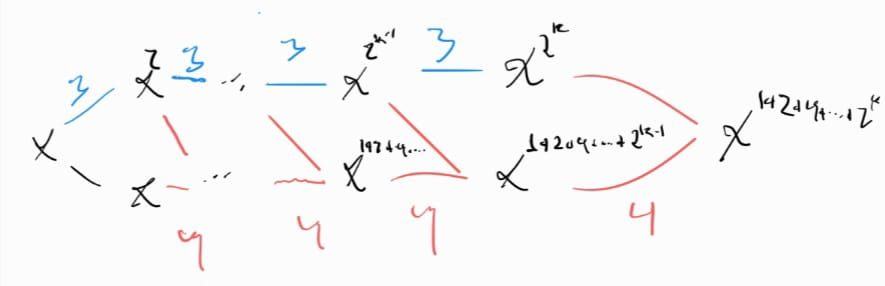
\includegraphics[width=0.8\textwidth]{fig/4.6.jpeg}
    \end{figure}
\end{frame}

\begin{frame}{Teo. 4.6}
    Essa construção leva $\lceil \log_2 d \rceil $ camadas e, no pior caso, $3+4=7$ neurônios por camada. \pause 

    \vspace{1em}

    Logo, $m^\text{Taylor}(x^d) \leq 7 \lceil \log_2 d \rceil$ 

    \pause
    \vspace{1em}

    Pela Prop. 3.3, sendo $x^d$ homogêneo, segue que $m^\text{uniform}(x^d) \leq m^\text{Taylor}(x^d). \blacksquare$

\end{frame}

\section{Como a eficiência melhora com a profundidade}
\begin{frame}
    \tableofcontents[currentsection]
\end{frame}

\begin{frame}{Teorema 5.1}
    \begin{teo}
        Seja $p(x) = x_1x_2 \dots x_n$ e suponha que $\sigma_i \neq 0$, para $i \leq n$. Então, 

        \begin{equation*}
            m_k^{uniform}(p) = \mathcal O(n^{\frac{k-1}{k}} 2^{n^{\frac 1 k}})
        \end{equation*}
    \end{teo}
\end{frame}

\begin{frame}{Conjectura 5.2}
    Seja $p(x) = x_1x_2 \dots x_n$ e suponha que $\sigma_i \neq 0$, para $i \leq n$. Então, 

        \begin{equation*}
            m_k^{uniform}(p) = 2^{\Theta (n^{\frac 1 k})},
        \end{equation*}
    
    i.e., o expoente cresce na ordem de $n^{\frac 1 k}$.
\end{frame}

\section{Referências}
\begin{frame}
\tableofcontents[currentsection]
\end{frame}

\begin{frame}
\frametitle{Referências}
\vspace{-2em}
\scriptsize
\bibliographystyle{abntex2-alf}
\bibliography{refs.bib}    
\end{frame}

\begin{frame}

\begin{center}
\Large Obrigado!
\end{center}

\vspace{1em}
Contato: riffel.felipe@grad.ufsc.br 

Repositório com os experimentos desenvolvidos: https://github.com/felipekriffel/TCC-Regularizacao-EIT
    
\end{frame}

\end{document}

